\documentclass[10pt]{article}

\usepackage{verbatim}
\usepackage{amsmath}
\usepackage{enumerate}
\usepackage{url}
\usepackage{geometry}
\usepackage{amsthm}
\usepackage{graphicx}

%\linespread{2}

%Title information for the entirety of the class document
\title{Hoverboard Construction and Experimentation using ROS}
\author{Kevin Chiang, Tony Schneider, Angela Yu, Baoliang Zhao}
\date{Due 9/26/2013}
\begin{document}
\maketitle

\section*{Introduction}
A robot can be thought of as a series of simple components working in unison to produce seemingly complicated behavior.  However, this requires each component to work as a cohesive whole -- a task which is daunting (to say the least). \emph {ROS} (the \textbf{R}obot \textbf{O}perating \textbf{S}ystem), an open source framework for robotics programming, was created to facilitate the use and communication of an arbitrary amount of these components (called \emph{nodes}). 

Using ROS in conjunction with several pre-written ROS nodes used to control radio and serial communication provides a platform for learning the basics of robotics. A hovercraft was constructed using relatively simple materials (i.e., styrofoam, tape, and plastic), and powered via 6 GW-EDF40 thrusters and a battery.  ROS was used to control each individual thruster with an Xbox controller, as well as fire thrusters in combination with one another to provide for more complicated translational movements.  This experience provided first hand experience in the construction and design of a simple robot, as well as an understanding of the fine tuning and manual evaluation required when working with mechanical systems.

\section*{Hovercraft Construction and Design}
The base of the hovercraft base was made of styrofoam roughly 1.5" thick.  A circular base was chosen for the simplicity of obtaining a balanced weight distribution and skirt construction.   The diameter of the base was 16.5".  The size of the base was chosen primarily because it was the size of the available template.  However, the size seems like a good compromise between a light weight and a surface area large enough to fit all of the individual components.  

The skirt was constructed by first drawing a circle 0.75 inches larger than the base with a spacer on the plastic sheeting.  The sheeting was then cut down, and taped to the bottom of the hovercraft.  Lastly, a circle 1.5 inches smaller than the base was drawn on the bottom sheet and cut out of the inner circle to create the skirt.  The first attempt resulted in a skirt that was too small due to a problem with taping the sheet to the base evenly, but the second attempt was a success.  

\begin{figure}
\centering
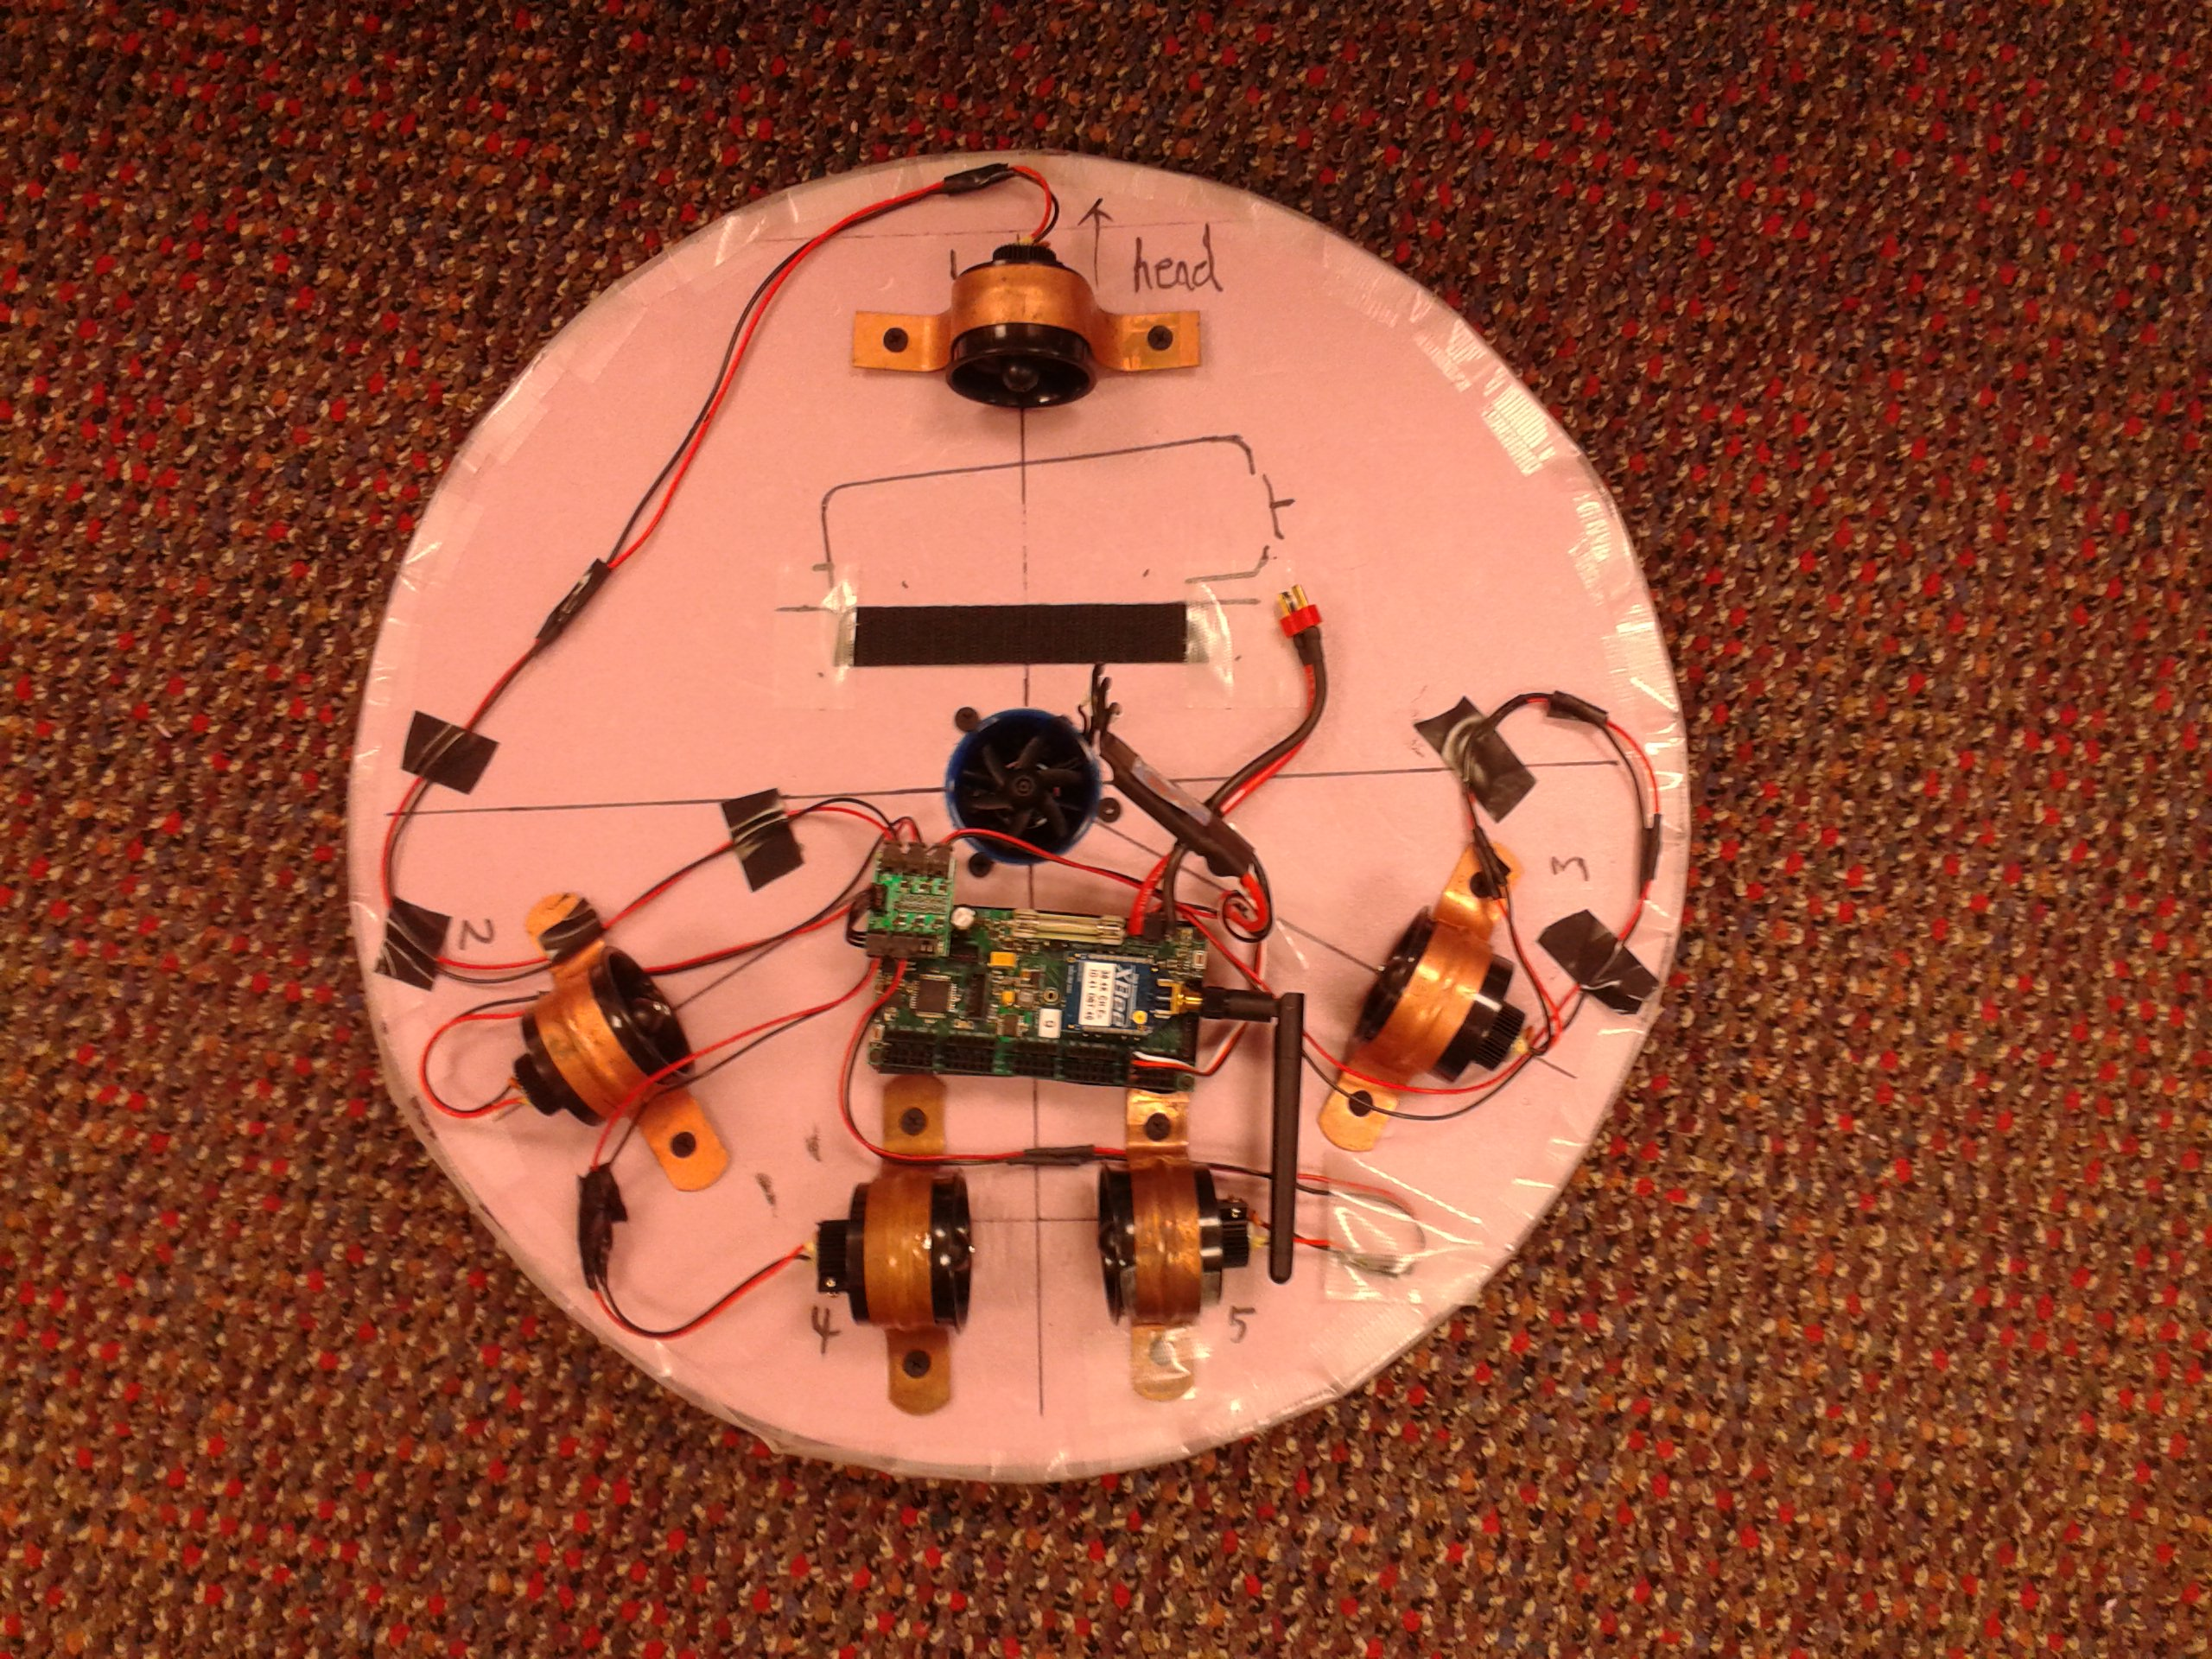
\includegraphics[width=.75\textwidth]{images/hovercraft}
\caption{Overhead view of the hovercraft after construction was completed}
\label{hovercraft}
\end{figure}

The configuration of the thrusters was adopted from the instructor's design.  The three translational thrusters were separated by 120� separation each around the circumference of the hovercraft (thrusters 1, 2, and 3 in figure~\ref{hovercraft}), and the two rotational thrusters are set in direct opposition to one another at the base of the craft (thrusters 4 and 5 in figure~\ref{hovercraft}). This design was adopted primarily for its relatively straightforward way of implementing left and right translation using two thrusters simultaneously (with a small amount of trigonometry), as well as the simplicity of rotation (i.e., by firing a single rotational thruster).  

This design required thrusters 1 and 3 to be relatively far away from the thrust controller on the hovercraft, so it was necessary to solder an extension to these thrusters.  However, thrusters 2, 4, and 5 were close enough to the controller that they could be attached without modifications.  The wires themselves were left unlabeled, but the thrusters corresponding to each input on the thrust controller were labeled with their corresponding connector number (as seen in figure~\ref{hovercraft}).

The positioning of the thrusters and board shifted the center of gravity of the hovercraft considerably.  To ameliorate this shift, the hoverboard controller and battery were mounted on the two sides of the lift thruster (center of figure~\ref{hovercraft}), to shift the center of gravity back towards the center of the hovercraft.  


\section*{ROS Setup and Experiments}
--  Essentially section 5

\section*{Hovercraft Experiments}
-- Essentially section 6

\end{document}